% !TeX spellcheck = de_CH
\chapter{Bellsche Ungleichung\label{chapter:bell}}
\lhead{Bellsche Ungleichung}
\begin{refsection}
\chapterauthor{Hannes Badertscher}

In diesem Kapitel betrachten wir ein Gedankenexperiment von Albert Einstein
genauer.
Wie Randall Munroe von xkcd im Comic~\ref{fig:bell:xkcd_einstein} illustriert,
konnten die Theorien von Einstein bisher selten widerlegt werden.
Als einziges Beispiel, Einstein zu widerlegen, wird eine m\"oglicherweise
falsche Entscheidung Einsteins aufgef\"uhrt, als er bei seiner Arbeit im
Patentamt ein umstrittenes Patent zur Annahme empfahl.
Obwohl scheinbar unm\"oglich, befassen wir uns in diesem Kapitel mit der Arbeit
von Albert Einstein und versuchen diese kritisch zu beleuchten.

\begin{figure}[b]
    \centering
    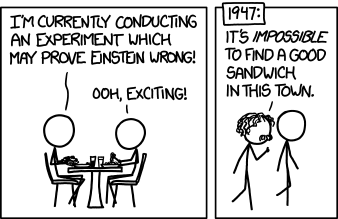
\includegraphics[width=0.5\linewidth]{bell/images/xkcd_einstein.png}
    \caption{XKCD Comic, welches darauf anspielt, dass sich kaum Fehler 
    in den Arbeiten von Albert Einstein finden lassen \cite{Bell:XkcdEinstein}}
    \label{fig:bell:xkcd_einstein}
\end{figure}

Im Mai 1935 ver\"offentlichten Albert Einstein, Boris Podolsky und
Nathan Rosen ein Gedankenexperiment mit welchem sie erkl\"arten, wieso
die Quantenmechanik nicht vollst\"andig sein kann. Als Alternative
sollten zus\"atzliche, verborgene Variablen eingef\"ugt werden, welche
das zugrunde liegende Verhalten logisch erkl\"aren k\"onnen.
W\"ahrend Niels Bohr die bisherige (Kopenhagen-) Interpretation der 
Quantenmechanik verteidigte, befassten sich diverse Physiker mit die Suche
nach solchen verborgenen Variablen.
In vielen Bereichen der Quantenmechanik wurden tats\"achlich
kleinere Teilchen, Quantenzahlen und Variablen entdeckt, welche das
Verst\"andnis der heutigen Quantenphysik pr\"agten.
Zur L\"osung des Gedankenexperiments von Einstein, Rosen und Podolsky konnten
jedoch bisher keine verborgenen Variablen gefunden werden.

Wir betrachten das Gedankenexperiment von Einstein, indem wir zuerst die
grundlegenden Annahmen der Lokalit\"at und des Realismus betrachten. Danach
gehen wir auf das von Einstein, Rosen und Podolski ver\"offentlichte Paradoxon
ein und kommen auf die darauf basierende Bellsche Ungleichung, welche
1961 von John Bell ver\"offentlicht wurde.

\section{Definitionen\label{section:bell:definitionen}}
Zuerst stellt sich die Frage der Anforderungen an die Theorie der
Quantenmechanik.
In diesem Abschnitt werden diese Begriffe Anforderungen kurz definiert und
besprochen, sodass diesbez\"uglich keine Unklarheiten entstehen.
Albert Einstein stellte dabei die folgenden beiden Anforderungen an eine
Theorie:

\begin{enumerate}
    \item Lokalit\"at
    \item Realismus
\end{enumerate}

Die zentrale Eigenschaft ist dabei die Lokalit\"at.
Dies bedeutet, dass jegliche Vorg\"ange nur einen Einfluss
auf ihre direkte Umgebung haben k\"onnen.

\begin{definition}\label{def:bell:lokalitaet}
    Eine physikalische Theorie ist \emph{lokal}, wenn zwei \"ortlich getrennte
    Systeme keinen sofortigen Einfluss aufeinander haben k\"onnen.
\end{definition}

\foreignquote{english}{Spooky actions at a distance} \cite[S.~158]{Bell:BornEinstein1971}
konnte sich Einstein nicht vorstellen.
Zum Beispiel war klassische Newtonsche Gravitationstheorie
eine \emph{nicht}-lokale Theorie. 
Eine Masse hat in der Gravitation sofort, ohne zeitliche 
Verz\"ogerung, einen Einfluss auf andere Massen -- unabh\"angig von der
r\"aumlichen Distanz zwischen den beiden Massen. 
In der speziellen Relativit\"atstheorie wurden die Begriffe von Raum und Zeit
so definiert, dass sich alle Materie und Energie h\"ochstens mit
Lichtgeschwindigkeit fortbewegen kann. 
Die allgemeine Relativit\"atstheorie ist eine alternative Formulierung
der Newtonschen Gravitationstheorie, welche die in der speziellen
Relativit\"atstheorie geforderte Lokalit\"at erf\"ullt.
Einstein war sich deshalb sicher, dass auf f\"ur die Quantenmechanik eine
Theorie herleiten l\"asst, in welcher sich jegliche Ereignisse h\"ochstens mit
Lichtgeschwindigkeit ausbreiten k\"onnen.

Mit der Forderung des Realismus wird verlangt, dass die Theorie eine
physikalische \emph{Realit\"at} beschreibt.
Das heisst dass eine Messung immer einen vorbestimmten Wert hat, und dieser
g\"ultig ist und existiert, ob die Messung durchgef\"uhrt wird oder nicht.

\begin{definition}\label{def:bell:}
    Eine physikalische Theorie ist \emph{realistisch}, wenn das Ergebnis
    jeglicher Messungen vorbestimmt ist.
\end{definition}

In einem Gespr\"ach mit Abraham Pais verdeutlichte Albert Einstein diese
Forderung mit dem bekannten Spruch
\foreignquote{english}{Do you really believe that the moon exists only when you look at it?}\cite{Bell:Pais1979}



\section{Das Einstein-Podolsky-Rosen Paradoxon\label{section:bell:epr}}
Das Einstein-Podolsky-Rosen Paradoxon (EPR Paradoxon) ist ein 
Gedankenexperiment, welches 1935 im Paper \cite{Bell:Einstein1935}
\enquote{Can quantum-mechanical description of physical reality be considered complete?}
von Albert Einstein, Boris Podolsky und Nathan Rosen publiziert wurde.
Einstein \emph{et al.} beginnen das Paper mit zwei Fragen zur
Quantenmechanik:

\begin{enumerate}
    \item Ist die Theorie korrekt?
    \item Ist die Beschreibung durch die Theorie vollst\"andig?
\end{enumerate}

Nur wenn beide diese Fragen mit \enquote{ja} beantwortet werden k\"onnen, 
ist die Theorie eine zufriedenstellende Beschreibung der Realit\"at.
Ob eine Theorie als korrekt bezeichnet werden kann wird definiert mit:

\begin{definition}\label{def:bell:Korrektheit}
    Die Korrektheit einer Theorie wird anhand des Grades der \"Ubereinstimmung
    zwischen den Vorhersagen einer Theorie und den entsprechenden praktischen
    Messungen und Experimenten.
\end{definition}

Diese Frage kann einfach gepr\"uft werden, indem die Resultate von
Experimenten mit den Vorhersagen der Theorie verglichen werden. 
Die Quantenmechanik konnte dabei, wie wir in diesem Buch in zahlreichen
Anwendungen nachvollziehen konnten, die Wirklichkeit korrekt vorhersagen. 
Um die zweite Frage zu diskutieren, definieren die Vollst\"andigkeit einer
Theorie wie folgt:

\begin{definition}\label{def:bell:Vollstaendigkeit}
    Jedes Element der physikalischen Realit\"at muss durch die Theorie
    genau beschrieben werden k\"onnen.
\end{definition}

Einstein, Podolsky und Rosen gehen in ihrem Paper genauer auf die Frage
der Vollst\"andigkeit der Quantenmechanik ein.
Dazu pr\"asentieren sie ein Gedankenexperiment, anhand welchem bewiesen
werden soll, dass die Quantenmechanik nicht vollst\"andig ist.
W\"ahrend Einstein \emph{et al.} das Gedankenexperiment sehr
allgemein hielten, diskutieren wir hier ein anschaulicheres Beispiel, welches
1957 von David Bohm und Yakir Aharonov \cite{Bell:Bohm1957} pr\"asentiert
wurde.

\subsection{Das Gedankenexperiment\label{subsection:bell:epr:idee}}
Wir betrachten zwei quantenmechanische Systeme, $I$ und $II$,
welche von $t=0$ bis zu einem Zeitpunkt $t=T$ miteinander 
interagieren k\"onnen. Darauf ist keine Interaktion mehr m\"oglich.
Visualisiert wird das Gedankenexperiment durch eine Quelle, welche
Elektron-Positron Paare emittiert. 
Dabei wird das Elektron (System $I$) zu einem Detektoren $A$ und das 
Positron (System $II$) zu einem Detektoren $B$ gesandt.
Diese sind physikalisch getrennt, sodass kein Informationsaustausch
zwischen den Detektoren m\"oglich ist.
Der Messaufbau ist in \figurename~\ref{fig:bell:EPR_Messaufbau} abgebildet.

\begin{figure}
    \centering
    \includegraphics{bell/images/experiment_setup.pdf}
    \caption{Messaufbau im Gedankenexperiment von EPR}
    \label{fig:bell:EPR_Messaufbau}
\end{figure}

Diese zwei Partikel werden so generiert, dass sie einen komplement\"aren
Spin-Zustand besitzen. 
Durch das Gesetz der Drehimpulserhaltung \textsuperscript{[Citation needed]}
ist dies einfach m\"oglich, da der Gesamtdrehimpuls eines Elektron-Positron Paares $+\frac12 - \frac12 = 0$ betr\"agt.

Wenn also bei Detektor $A$ der Spin des Elektrons entlang der $z$-Achse
gemessen wird und das Messresultat $+z$ ist, so ist sofort klar, dass
das das Positron bei Detektor $B$ den Spin $-z$ besitzen muss. 
Ebenso wird, falls bei Detektor $A$ der Spin entlang der $x$-Achse als $+x$
gemessen wird, das Positron bei Detektor $B$ den Spin $-x$ besitzen.

Wie im Kapitel der Heisenbergschen Unsch\"arferelation 
(Kapitel~\ref{chapter:heisenberg})
erkl\"art wird, sind die Messungen des Spins in verschiedenen Dimensionen 
komplement\"are Operatoren.
Damit ist es unm\"oglich, gleichzeitig beide Eigenschaften eines Teilchens
beliebig genau zu kennen.
Wird nun jedoch bei Detektor $A$ der Spin des Elektrons in $z$-Richtung 
als $+z$ gemessen, so ist bekannt dass das Positron den Spin $-z$ besitzt.
Da jedoch noch keine Messung am Positron ausgef\"uhrt wurde, kann bei
Detektor $B$ der Spin in $x$-Richtung gemessen werden.
Es ist also m\"oglich f\"ur das Positron gleichzeitig die exakten Werte 
des Spins in $x$-, wie in $z$-Richtung zu kennen. 
Mit der uns bekannten Beschreibung der Quantenmechanik mit Wellenfunktionen
kann dieser Effekt \emph{nicht} beschrieben werden, womit wir zu der
logischen Schlussfolgerung Einsteins kommen:

\begin{satz}
    Die quantenmechanische Beschreibung der physikalischen Realit\"at mittels
    Wellenfunktionen ist keine vollst\"andige Theorie.
\end{satz}

\subsection{Mathematische Herleitung\label{subsection:bell:epr:herleitung}}
Anhand des Spins kann das EPR Paradoxon einfach mathematisch formuliert werden.
Dabei wird die Notation aus Kapitel~\ref{chapter:spin} (\nameref{chapter:spin})
verwendet.

Wie in den Gleichungen~\ref{spin:paulimatrizen}--\ref{spin:vektoroperator}
hergeleitet wird der Spin-Operator durch die hermiteschen Pauli-Matrizen
beschrieben.

\begin{align}
    S_x &= \frac{\hbar}{2} \begin{pmatrix}
    0 & 1 \\ 1 & 0
    \end{pmatrix}
    &
    S_y &= \frac{\hbar}{2} \begin{pmatrix}
    0 & -i \\ i & 0
    \end{pmatrix}
    &
    S_z &= \frac{\hbar}{2} \begin{pmatrix}
    1 & 0 \\ 0 & -1
    \end{pmatrix}\label{equ:bell:paulimatrizen}
\end{align}

Wie in Abschnitt~\ref{subsection:bell:epr:idee} erkl\"art, betrachten wir
den Spin in $x$- und $z$-Richtung.
Die Eigenwerte der entsprechenden Pauli-Matrizen betragen:

\begin{align}
    |{+}x\rangle &= \frac{1}{\sqrt{2}}\begin{pmatrix} 1\\1 \end{pmatrix} &
    |{-}x\rangle &= \frac{1}{\sqrt{2}}\begin{pmatrix} 1\\-1 \end{pmatrix} &
    |{+}z\rangle &= \begin{pmatrix} 1\\0 \end{pmatrix} &
    |{-}z\rangle &= \begin{pmatrix} 0\\1 \end{pmatrix} &
\end{align}

Der Spin-Zustand $|\psi\rangle$ entlang der $z$-Achse eines 
Elektron-Positron Paares  kann durch alle m\"oglichen Kombination der beiden
Spins von Elektron und Positron beschrieben werden. 
Diese umfassen $+z$ f\"ur das Elektron und $-z$
f\"ur das Positron, sowie $-z$ f\"ur das Elektron und $+z$ f\"ur das Positron.
Zur Notation dieser kombinierten Zust\"ande wird das Tensorprodukt verwendet.

\begin{definition}\label{def:bell:tensorprodukt}
    Das Tensorprodukt von zwei Vektoren $A,B \in \mathbb{C}^2$  wird geschrieben als
    \[
        A \otimes B
    \]
    und entspricht der Abbildung $(\mathbb{C}^2,\mathbb{C}^2)\to\mathbb{C}^4$, 
    bei welcher jedes Element von $A$ mit jedem Element von $B$ multipliziert
    wird.
    Seien
    \begin{align*}
        A = \begin{pmatrix} a_{1} \\ a_{2} \end{pmatrix}
        &&
        B = \begin{pmatrix} b_{1} \\ b_{2} \end{pmatrix}
    \end{align*}
    so entspricht das Tensorprodukt
    \[
        A \otimes B = \begin{pmatrix} 
        a_1 b_1 \\ a_1 b_2 \\ a_2 b_1 \\ a_2 b_2
        \end{pmatrix}
    \]
\end{definition}

Damit ist der Zustand des Systems $|\psi\rangle$ definiert als

\begin{equation}
    |\psi\rangle = \frac{1}{\sqrt{2}} \Big( 
        |{+}z\rangle \otimes |{-}z\rangle - |{-}z\rangle \otimes |{+}z\rangle
     \Big)
     \label{equ:bell:spinstate}
\end{equation}

und somit

\begin{align}
    |\psi\rangle &= \frac{1}{\sqrt{2}} 
    \left( 
        \begin{pmatrix} 1\\0 \end{pmatrix} 
        \otimes 
        \begin{pmatrix} 0\\1 \end{pmatrix}
        -
        \begin{pmatrix} 0\\1 \end{pmatrix}
        \otimes
        \begin{pmatrix} 1\\0 \end{pmatrix}
     \right)
     =
     \frac{1}{\sqrt{2}}\left(
         \begin{pmatrix} 0 \\ 1 \\ 0 \\ 0 \end{pmatrix}
         -
         \begin{pmatrix} 0 \\ 0 \\ 1 \\ 0 \end{pmatrix}
     \right)
     \stackrel{!}{=}
     \frac{1}{\sqrt{2}}\left(
         \frac{1}{2}
         \begin{pmatrix} \phantom{-}1 \\ \phantom{-}1 \\ -1 \\ -1 \end{pmatrix}
         -
         \frac{1}{2}
         \begin{pmatrix} \phantom{-}1 \\ -1 \\ \phantom{-}1 \\ -1 \end{pmatrix}
     \right)  \notag \\
     &=
    -\frac{1}{\sqrt{2}} \left( 
        \frac{1}{\sqrt{2}}\begin{pmatrix} 1 \\ 1 \end{pmatrix} 
        \otimes 
        \frac{1}{\sqrt{2}}\begin{pmatrix} \phantom{-}1 \\ -1 \end{pmatrix}
        -
        \frac{1}{\sqrt{2}}\begin{pmatrix} \phantom{-}1 \\ -1 \end{pmatrix}
        \otimes
        \frac{1}{\sqrt{2}}\begin{pmatrix} 1 \\ 1 \end{pmatrix} 
     \right) \notag  \\
      &= 
      -\frac{1}{\sqrt{2}} \Big( 
              |{+}x\rangle \otimes |{-}x\rangle - |{-}x\rangle \otimes |{+}x\rangle
           \Big)\label{equ:bell:psix}
\end{align}

Wir haben also gezeigt, dass mit der Spin-Zustand $|\psi\rangle$ des
Elektron-Positron Paares \"aquivalent in Abh\"angigkeit des $z$-, sowie
des $x$-Spin Zustands geschrieben werden kann.
Wird nun bei Detektor $A$ der Spin des Elektrons in $z$-Richtung gemessen, 
so findet eine Projektion des Zustands $|\psi\rangle$ auf entweder
$|{+}z\rangle$ oder $|{-}z\rangle$ statt.
Der Zustand reduziert sich auf
\begin{align*}
    |\psi_{1}\rangle &= |{+}z\rangle \otimes |{-}z\rangle
    & \text{bzw.} && 
    |\psi_{2}\rangle &= |{-}z\rangle \otimes |{+}z\rangle
\end{align*}
Damit ist der Spin in $z$-Richtung f\"ur das Positron bei Detektor $B$ ohne
eine Messung vorbestimmt, n\"amlich als $-z$ im ersten Fall bzw. $+z$ im
zweiten Fall.
Wenn nun bei Detektor $B$ der Spin des Positrons in $x$-Richtung gemessen
wird, so wird der urspr\"ungliche Spin-Zustand $|\psi\rangle$
ebenfalls reduziert auf
\begin{align*}
    |\psi_{a}\rangle &= |{+}x\rangle \otimes |{-}x\rangle
    & \text{bzw.} && 
    |\psi_{b}\rangle &= |{-}x\rangle \otimes |{+}x\rangle
\end{align*}
Wir erhalten damit zwei Wellenfunktionen, z.B. $|\psi_{1}\rangle$ und 
$|\psi_{a}\rangle$, welche \emph{gleichzeitig} die gleiche 
physikalische Realit\"at beschreiben.
Um zu pr\"ufen ob dies im Fall des Spin-Zustands \"uberhaupt m\"oglich 
ist, wenden wir Hilfssatz~\ref{skript:kommutatorannihliertev} an.
Der Kommutator $[S_x,S_z]$ ist
\begin{equation}
    [S_x, S_z] =  -i \hbar S_y \neq 0
\end{equation}
Da die Operatoren $S_x$ und $S_z$ also nicht vertauschen, ist nach der Theorie
der Quantenmechanik die gleichzeitige Kenntnis der beiden Messungen nicht
m\"oglich.
Dass dies jedoch hier der Fall ist, haben wir in Abschnitt~\ref{subsection:bell:epr:idee}
hergeleitet und mathematisch in diesem Abschnitt beweisen k\"onnen.
Damit m\"ussen wir zur Schlussfolgerung kommen, dass entweder 
(1) eine sofortige Kommunikation zwischen dem Elektron und dem Positron
stattfindet, was  jedoch durch die Lokalit\"at ausgeschlossen wird,
oder (2) dass die Beschreibung der Quantenmechanik mittels der Wellenfunktion
nicht  vollst\"andig ist und ein fundamentaler, nicht messbarer, Mechanismus
bestimmt welches Ergebnis eine Messung des Spins ergeben wird.


\subsection{Die Theorie der verborgenen lokalen Variablen}
Besinnen wir uns zur\"uck auf die beiden initialen Fragen: 
(1) \enquote{Ist die Theorie korrekt?} und 
(2) \enquote{Ist die Beschreibung durch die Theorie vollst\"andig?}
Dabei mussten wir feststellen, dass zwar die Frage (1) dank diverser
Experimente mit \enquote{ja} beantwortet werden kann, doch die Frage (2) 
durch das besprochene Gedankenexperiment nur mit \enquote{nein} beantwortet
werden kann. 
Damit stellt sich die Frage, um welches Element die Theorie der Quantenmechanik
erweitert werden muss, sodass die Beschreibung vollst\"andig wird.

Ein Ansatz, welcher dabei auf der Hand liegt, wurde in
Abschnitt~\ref{subsection:bell:epr:herleitung} bereits angeschnitten: 
Es muss ein verborgener Mechanismus existieren, welcher das Resultat unseres
Experiments, also den Spin von Elektron und Positron, vorausbestimmt.
Dazu wird eine verborgene Variable $\lambda$ eingef\"uhrt.
$\lambda$ wird als \emph{verborgene} Variable bezeichnet, da diese nicht
messbar ist, sondern nur die Auswirkungen der Variable, also der jeweilige
Spin, gemessen werden kann.
Um das durch Einstein, Rosen und Podolski eingef\"uhrte Paradoxon zu l\"osen
reicht eine 2-dimensionale Variable aus, welche den Zusammenhang zwischen
dem Spin in $x$- und $z$-Richtung beschreibt.
Eine Visualisierung der m\"oglichen Werte von $\lambda$ ist in 
Abbildung~\ref{fig:bell:hidden_var} dargestellt.

\begin{figure}
    \centering
    \includegraphics{bell/images/hidden_vars.pdf}
    \caption{Visualisierung der verborgenen Variable $\lambda$ des Spin-Zustands}
    \label{fig:bell:hidden_var}
\end{figure}

Liegt die Variable $\lambda$ des Positrons im ersten Quadranten des Diagramms,
so ist unabh\"angig von der Messung des Elektrons bei Detektor $A$ eindeutig
bestimmt, dass der Spin in $x$- und in $z$-Richtung positiv sein wird. 
$\lambda$ ist jedoch nicht direkt messbar, es muss also trotzdem der Spin
in $z$-Richtung bei Detektor $A$ und in $x$-Richtung bei Detektor $B$ gemessen
werden, um den Wert von $\lambda$ bestimmen zu k\"onnen.
Da der Wert von $\lambda$ in der Quelle, beim Generieren des Elektron-Positron
Paares gesetzt wird und danach nicht ver\"andert wird, wird sich $\lambda$
an die Forderung der Lokalit\"at halten.
\enquote{Spukhafte Fernwirkungen}, wie Einstein die Beobachtungen seines
Gedankenexperiments nannte, werden damit ausgeschlossen und die Theorie
der Quantenmechanik wird so erweitert, dass sie \emph{vollst\"andig} ist.
Die Herausforderung eine solche lokale, verborgene Variable $\lambda$ wirklich 
in Form eines existierenden Teilchens zu finden bleibt jedoch bestehen.

\section{Die Bell'sche Ungleichung\label{section:bell:bell}}
%http://arxiv.org/pdf/quant-ph/0509061.pdf
Nach der Ver\"offentlichung des EPR Paradoxons gingen verschiedene bekannte
Physiker auf das Paradoxon ein.
Der gr\"osste Verfechter der Quantenmechanik, Niels Bohr, antwortete bereits
1935 mit einer eher schwammigen Widerlegung Einsteins, welche weitere 
Anh\"anger der Quantenmechanik zu jener Zeit bereits zufriedenstellte
\textsuperscript{[Citation needed]}.
Im Nachhinein betrachtet musste 1949 sogar Bohr selbst zugeben, dass seine
Reaktionen auf Einstein \enquote{ineffizient} waren und 
\enquote{es schwierig machten darauf zu antworten}. 
Erwin Schr\"odinger hingegen zweifelte nicht am EPR Paradoxon selbst, sondern
daran, dass sich die Erkenntnisse der Quantenmechanik auf die makroskopische
Welt \"ubertragen lassen, und somit ob der Effekt auch messbar sei.
Dies \"ausserte er insbesondere im ber\"uhmten Paradoxon von 
Schr\"odingers Katze, welches in Abbildung~\ref{fig:bell:xkcd_schroedinger}
verdeutlicht wird \textsuperscript{[Citation needed]}.

\begin{figure}
    \centering
    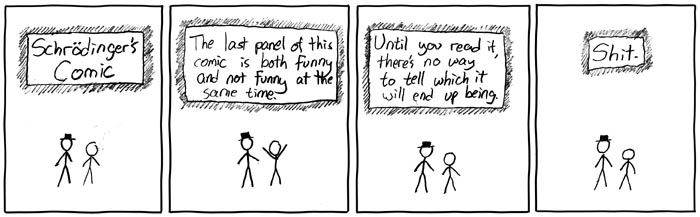
\includegraphics[width=0.8\linewidth]{bell/images/xkcd_schroedinger.jpg}
    \caption{xkcd Comic zum Paradoxon Schr\"odingers Katze, welches daran
    zweifelt, dass sich Quantenmechanische Effekte auf die makroskopische
    Welt \"ubertragen lassen. \cite{Bell:XkcdSchroedinger}}
    \label{fig:bell:xkcd_schroedinger}
\end{figure}

David Bohm hingegen versuchte das Gedankenexperiment Einsteins zu verteidigen
\textsuperscript{[Citation needed]}.
Er entwickelte dazu eine dem EPR-Experiment sehr \"ahnliche Idee, indem er
nicht Position und Drehmoment, sondern den Spin zweier Partikel betrachtete.
Dieses Gedankenexperiment ist einfacher zu analysieren (weshalb wir im
Abschnitt~\ref{section:bell:epr} das Experiment von Bohm, und nicht das
originale von Einstein betrachtet haben), und ist experimentell einfacher
zu pr\"ufen.

Als sich John Bell, noch als Student, mit dem EPR Paradoxon und insbesondere
der Arbeit von David Bohm zu besch\"aftigen begann, war er \"uberzeugt von
der Theorie der verborgenen lokalen Variablen zur L\"osung des EPR Paradoxons
\textsuperscript{[Citation needed]}.
Er besch\"aftigte sich insbesondere mit der Frage, ob eine solche Theorie
\"uberhaupt eine Lokalit\"at zul\"asst, oder ob die Annahme Bohms,
dass eine lokale Quantenmechanik nicht m\"oglich ist, zutrifft.
Obwohl \"uberzeugt von verborgenen lokalen Variablen, gelang es Bell 1964
in seinem Paper 
\enquote{On the Einstein Podolsky Rosen Paradox} \cite{Bell:Bell1964}
zu beweisen, dass eine Theorie der verborgenen Variablen -- sollte eine
solche existieren -- \emph{nicht} lokal sein kann.
Als erstem Physiker gelang es die Frage umzudrehen, und nicht nach solchen
Variablen bzw. Teilchen zu suchen, sondern gleich deren Nicht-Existenz
zu beweisen.

\subsection{Vorhersage der Quantenmechanik}
Der Spin eines Teilchens in einer Richtung $\vec{a}$ wird durch die Projektion
der Spin-Matrix des Teilchens $A$ auf die Richtung $\vec{a}$ gemessen.
\begin{equation}\label{equ:bell:meas_a}
    \vec{\hat{\sigma}}_A \cdot \vec{a}
\end{equation}
Dies kann mithilfe der Pauli-Matrizen \eqref{equ:bell:paulimatrizen} geschrieben
werden als
\begin{align}
    \vec{a} \cdot \vec{\hat{\sigma}}_A &= 
    a_1 \hat{\sigma}_x + a_2 \hat{\sigma}_y + a_3 \hat{\sigma}_z = 
    a_1 \begin{pmatrix} 0 & 1 \\ 1 & 0 \end{pmatrix} +
    a_2 \begin{pmatrix} 0 & -i \\ i & 0 \end{pmatrix} + 
    a_3 \begin{pmatrix} 1 & 0 \\ 0 & -1 \end{pmatrix} \\
    & = \begin{pmatrix}
       a_3 & a_1 - i a_2 \\
       a_1 - i a_2 & -a_3
    \end{pmatrix} \label{equ:bell:proj_a_s}
\end{align}
Der Spin-Zustand $|\psi\rangle$ des Elektron-Positron Paares kann mit
\eqref{equ:bell:meas_a} und gleich f\"ur das Teilchen $B$: 
$\vec{\hat{\sigma}}_B \cdot \vec{b}$ als Superposition der beiden
Spin-Zust\"ande bei $A$ und $B$ geschrieben werden:
\begin{equation}
    |\psi\rangle = \left( \vec{\hat{\sigma}}_A \cdot \vec{a} \right)
        \otimes \left( \vec{\hat{\sigma}}_B \cdot \vec{b} \right)
\end{equation}
Der Erwartungswert $E_{QM}$ des Produkts der zwei Spin-Messungen
ist daher
\begin{equation}\
    E_{QM} = \left\langle \phi \left| 
    \left( \vec{\hat{\sigma}}_A \cdot \vec{a} \right)
            \otimes \left( \vec{\hat{\sigma}}_B \cdot \vec{b} \right)
    \right| \phi \right\rangle
\end{equation}
Da die Messung jeweils entweder $|+\rangle$ oder $|-\rangle$ ergibt, kann
dies analog zu \eqref{equ:bell:spinstate} umgeformt werden.
\begin{equation} 
\begin{split}
   E_{QM }=&\left\langle \phi \left| 
       \left( \vec{\hat{\sigma}}_A \cdot \vec{a} \right)
               \otimes \left( \vec{\hat{\sigma}}_B \cdot \vec{b} \right)
       \right| \phi \right\rangle
    = \\
    \frac{1}{2}\Bigg[ &
        \left\langle{+}\left| \vec{\hat{\sigma}}_A \cdot \vec{a} \right|{+}\right\rangle_A
        \left\langle{-}\left| \vec{\hat{\sigma}}_B \cdot \vec{b} \right|{-}\right\rangle_B
        -
        \left\langle{+}\left| \vec{\hat{\sigma}}_A \cdot \vec{a} \right|{-}\right\rangle_A
        \left\langle{-}\left| \vec{\hat{\sigma}}_B \cdot \vec{b} \right|{+}\right\rangle_B \\
        - &
        \left\langle{-}\left| \vec{\hat{\sigma}}_A \cdot \vec{a} \right|{+}\right\rangle_A
        \left\langle{+}\left| \vec{\hat{\sigma}}_B \cdot \vec{b} \right|{-}\right\rangle_B
        +
        \left\langle{-}\left| \vec{\hat{\sigma}}_A \cdot \vec{a} \right|{-}\right\rangle_A
        \left\langle{+}\left| \vec{\hat{\sigma}}_B \cdot \vec{b} \right|{+}\right\rangle_B
    \Bigg]
\end{split}
\end{equation}
Was mit \eqref{equ:bell:proj_a_s} vereinfacht werden kann zu
\begin{equation}\label{equ:bell:e_qm}
\begin{split}
    E_{QM} &= \frac{1}{2} \big[ -a_3b_3 - (a_1-ia_2)(b_1+ib_2) - (a_1+ia_2)(b_1-ib_2) - a_3b_3 \big] \\
    &= -\big[ a_1b_1 + a_2b_2 + a_3b_3 \big] \stackrel{!}{=} -\vec{a} \cdot \vec{b}
\end{split}
\end{equation}
Da $\vec{a}$ und $\vec{b}$ Einheitsvektoren sind, gilt
\begin{equation}
    \vec{a} \cdot \vec{b} = \cos(\theta_{ab}) \qquad \text{f\"ur} \quad |\vec{a}| = |\vec{b}| = 1
\end{equation}
mit dem Winkel $\theta_{ab}$ zwischen $\vec{a}$ und $\vec{b}$.
Somit wird der quantenmechanische Erwartungswert zu
\begin{equation}
    E_{QM}(\vec{a},\vec{b}) = -\vec{a}\cdot\vec{b} = -\cos(\theta_{ab})
\end{equation}

\subsection{Vorhersage mittels verborgener Variablen}
Nehmen wir nun an, dass eine Theorie der verborgenen Variablen vorliegt
und eine Variable $\lambda \in \Lambda$ existiert.
\"Uber die Art dieser Variable, ob kontinuierlich oder diskret, wird hier keine
Annahme gemacht.
Die Wahrscheinlichkeitsverteilung dieser Variable sei $\rho(\lambda)$, womit gilt
\begin{equation}\label{equ:bell:lambdaverteilung}
    \int_{\lambda\in\Lambda} \rho(\lambda) d\lambda
\end{equation}

Damit diese Theorie die Quantenmechanik erweitern kann, muss sie die Vorhersage
der Quantenmechanik mit dem Erwartungswert 
$E_{QM}(\vec{a},\vec{b}) = -\vec{a}\cdot\vec{b}$
ebenfalls f\"ur alle Richtungen $\vec{a}$ und $\vec{b}$ produzieren.

Die Messungen $A(\vec{a})$ und $B(\vec{b})$ h\"angen nun also von einer
vorbestimmten Variable $\lambda$ ab.
\begin{equation}\label{equ:bell:messungen_ab}
    A(\vec{a}) \cdot B(\vec{b})(\lambda) = A(\vec{a},\lambda) \cdot B(\vec{b},\lambda)
\end{equation}
mit
\[
    A(\vec{a},\lambda) = \pm 1 \qquad \text{und} \qquad B(\vec{b},\lambda) = \pm 1
\]
Aus \eqref{equ:bell:lambdaverteilung} und \eqref{equ:bell:messungen_ab}
l\"asst sich der Erwartungswert des Produkts der beiden Spin-Messungen
bestimmen als
\begin{equation}
    E(\vec{a},\vec{b}) = \int_{\lambda\in\Lambda} 
    \rho(\lambda) A(\vec{a},\lambda) B(\vec{b},\lambda) d\lambda
\end{equation}




\subsection{Herleitung der CHSH Ungleichung}
Wir bezeichnen das Resultat der Messung $a$ als $s$ und das Resultat
der Messung $b$ als $t$.
Nun definieren wir die Wahrscheinlichkeit, dass die Messung $a$ f\"ur ein
gegebenes $\lambda$ das Resultat $s$ ergibt, gegeben dass die Messung $b$ das
Resultat $t$ ergeben hat als $p_{\lambda}^1(s \mid a,b,t)$.
Gleich definieren wir als $p_{\lambda}^2(t \mid a,b,s)$ die Wahrscheinlichkeit
dass die Messung $b$ das Resultat $t$ ergibt, f\"ur ein gegebenes $\lambda$ und
das Resultat $t$ bei Messung $a$. 
Wir m\"ochten daraus die Wahrscheinlichkeit berechnen, dass die Messungen
$a$ und $b$ die Resultate $s$ und $t$ mit $s,t \in [-1,1]$ ergeben. 
Unter der Annahme, dass die Messungen $a$ und $b$ unabh\"angig sind und sich
nicht gegenseitig beeinflussen k\"onnen -- was in einer lokalen Theorie
aufgrund der Distanz der Teilchen gegeben sein muss -- kann diese geschrieben
werden als
\begin{equation}
    p_{\lambda}(s,t \mid a,b) 
    = p_{\lambda}^1(s \mid a,b,t) p_{\lambda}^2(t \mid a,b,s)
    = p_{\lambda}^1(s \mid a) p_{\lambda}^2(t \mid b)
    \label{equ:bell:wkeit}
\end{equation}

Der Erwartungswert der Ergebnisse $s,t$ wird damit zu
\begin{equation}
    E_{\lambda}(a,b) = \sum_s \sum_t p_{\lambda}(s,t \mid a,b) (st)
    \label{equ:bell:erwartungswert}
\end{equation}

Zur Herleitung der Bell'schen Ungleichung aus \eqref{equ:bell:wkeit} und
\eqref{equ:bell:erwartungswert} f\"uhren wir den
Hilfssatz~\ref{hilfssatz:bell:interval} ein.

\begin{hilfssatz}
    F\"ur die Variablen $q, q', r, r' \in [-1,1]$ liegt 
    $S \equiv qr + qr' + q'r - q'r'$ im geschlossenen Intervall $[-2,2]$.
    \label{hilfssatz:bell:interval}
\end{hilfssatz}
\begin{proof}[Beweis]
    $S$ ist linear in allen vier Variablen $q, q', r, r'$.
    Damit liegen das Maximum und das Minimum von $S$ an je einer der Ecken des
    Definitionsbereichs. Damit sind
    \begin{align*}
        S_{\text{min}} = (-1) + (-1) + (-1) - 1 = -4 &&
        S_ {\text{max}} = 1 + 1 + 1 - (-1) = 4
    \end{align*}
    Jedoch kann $S$ geschrieben werden als
    \[
        S = (q + q')(r + r') - 2 q'r'.
    \]
    Da die Extremstellen an den Grenzen, also $+1$ bzw. $-1$ f\"ur jede der
    Variablen, liegen muss, k\"onnen die Terme $(q+q')$ und $(r+r')$ nun nur
    die Werte $-2, 0, +2$ annehmen, w\"ahrend der Term $2q'r'$ 
    entweder $-2$ oder $+2$ betr\"agt.
    Damit sind f\"ur $S$ die Werte $\pm 3$ und $\pm 4$ an den Grenzen der
    Definitionsbereiche \emph{nicht} m\"oglich und $S$ wird den Wertebereich
    $[-2,2]$ haben.
\end{proof}

Wir definieren nun die in Hilfssatz~\ref{hilfssatz:bell:interval} erw\"ahnten
Gr\"ossen $q,q',r,r'$ als
\begin{align}
    q  &= \sum_s s p_{\lambda}^1 (s \mid a)  \label{equ:bell:q}\\
    q' &= \sum_s s p_{\lambda}^1 (s \mid a') \\
    r  &= \sum_t t p_{\lambda}^2 (t \mid b)  \\
    r' &= \sum_t t p_{\lambda}^2 (t \mid b') \label{equ:bell:rs}
\end{align}
Nun setzen wir \eqref{equ:bell:q}-\eqref{equ:bell:rs} in $S$ aus 
Hilfssatz~\ref{hilfssatz:bell:interval} ein und vereinfachen dies mithilfe von
\eqref{equ:bell:erwartungswert}
\begin{equation}
    -2 \leq E_{\lambda}(a,b) + E_{\lambda}(a,b') + E_{\lambda}(a',b) - E_{\lambda}(a',b') \leq +2
    \label{equ:bell:ineq1}
\end{equation}
Nun nutzen wir die Tatsache, dass die verborgene Variable $\lambda$ ebenfalls
mit einer Wahrscheinlichkeitsdichte $\rho(\lambda)$ mit 
$\lambda \in \Lambda$ beschrieben werden kann.
Die Wahrscheinlichkeit der Ereignisse $s$ und $t$ wird damit zu
\begin{equation}
    p_{\rho}(s,t  \mid a,b) = \int_{\Lambda} p_{\lambda}(s,t \mid a,b) d\rho
\end{equation}
mit Erwartungswert
\begin{equation}
    E_{\rho}(a,b) = \int_{\Lambda} E_{\lambda}(a,b) d\rho 
    = \sum_s \sum_t \int_{\Lambda} p_m(s,t \mid a,b) (st) \:d\rho
    \label{equ:bell:ew}
\end{equation}
Dies in \eqref{equ:bell:ineq1} eingesetzt ergibt
\begin{equation}
    -2 \leq E_{\rho}(a,b) + E_{\rho}(a,b') + E_{\rho}(a',b) - E_{\rho}(a',b') \leq +2
    \label{equ:bell:bellineq}
\end{equation}
Die Ungleichung \eqref{equ:bell:bellineq} wird nun als
\enquote{Bell-Clauser-Horne-Shimony-Holt (BCHSH) Ungleichung} bezeichnet
\textsuperscript{[Citation needed]}.

Nun verbinden wir diese Herleitung mit dem Resultat \eqref{equ:bell:bellineq}
mit dem in Abbildung~\ref{fig:bell:EPR_Messaufbau} dargestellten Messaufbau.
Betrachten wir erneut das Elektron-Positron Paar mit dem in
\eqref{equ:bell:spinstate} hergeleiteten Spin-Zustand
\begin{equation*}
    |\psi\rangle = \frac{1}{\sqrt{2}} \Big( 
        |{+}z\rangle \otimes |{-}z\rangle - |{-}z\rangle \otimes |{+}z\rangle
     \Big)
\end{equation*}
F\"ur zwei Messungen $a$ und $b$ mit jeweils einem fixen Winkel $\theta_s$ bzw.
$\phi_t$ zur $xy$-Ebene wird dies verallgemeinert zu
\begin{equation}
    |\psi\rangle = \frac{1}{\sqrt{2}} \Big(
        |\theta_{+1}\rangle_A |\theta_{-1}\rangle_B + |\theta_{-1}\rangle_A |\theta_{+1}\rangle_B
    \Big)
\end{equation}
Die Wahrscheinlichkeit der Messung von $s$ und $t$ ist
\begin{equation}
    P_{\psi}(s,t \mid a,b) = 
    \Big| \langle \psi \; |\theta_s \rangle_A \; |\phi_t\rangle_B\Big|^2
    \label{equ:bell:prob_st}
\end{equation}
Da $|\theta_{+1}\rangle_A$ und $|\theta_{+1}\rangle_B$ orthogonal sind und
das Produkt $|\theta_{+1}\rangle_A|\theta_{-1}\rangle_B = 1$ betragen muss,
kann \eqref{equ:bell:prob_st} f\"ur den Fall $s=1,t=-1$ vereinfacht werden zu
\[
    P_{\psi}(1,-1 \mid a,b) = 
    \frac{1}{2} \; \Big| {}_B\langle \theta_1 \mid \phi_{-1} \rangle_B  \ \Big|^2
\]

Um diese Wahrscheinlichkeit berechnen zu k\"onnen, wird ohne Beweis der
Hilfssatz~\ref{hilfssatz:bell:malus} eingef\"uhrt
\textsuperscript{[Citation needed]}.

\begin{hilfssatz}\label{hilfssatz:bell:malus}
    Das Gesetz von Malus, welches die Transmission einer polarisierten
    Strahlung durch einen idealen Polarisator beschreibt: 
    $I = I_0 \cos^2(\alpha)$, gilt ebenfalls f\"ur Elektronen und Positronen
    mit dem jeweiligen Spin.
\end{hilfssatz}

Damit wird die Wahrscheinlichkeit $P_{\psi}(1,-1 \mid a,b)$ mit dem Winkel
$\sigma$ zwischen $a$ und $b$ zu
\begin{equation}
    P_{\psi}(1,-1 \mid a,b) = \frac{1}{2} \cos^2\sigma
\end{equation}
Genau gleich werden die Wahrscheinlichkeiten von $s=-1,t=1$, sowie
$s=t=1$ und $s=t=-1$ berechnet:
\begin{align}
    P_{\psi}(-1,1 \mid a,b) &= \frac{1}{2} \cos^2\sigma \\
    P_{\psi}(1,1 \mid a,b) &= \frac{1}{2} \sin^2\sigma \\
    P_{\psi}(-1,-1 \mid a,b) &= \frac{1}{2} \sin^2\sigma
\end{align}
Der Erwartungswert $E_{\psi}$ wird damit zu
\begin{align}
    E_{\psi}(a,b) &= P_{\psi}(1,-1 \mid a,b) + P_{\psi}(-1,1 \mid a,b) -
        P_{\psi}(1,1 \mid a,b) - P_{\psi}(-1,-1 \mid a,b)  \notag \\
    &= \cos^2\sigma - \sin^2\sigma  = \cos 2\sigma
\end{align}
%TODO: aber das ist für photonen?!?!

Nun werden betrachten wir die konkreten Werte 
$a=\frac{\pi}{4}, a'=0, b=\frac{\pi}{8}, b' = \frac{3\pi}{8}$ 
und setzen diese in \eqref{equ:bell:bellineq} ein. Wir erhalten
\begin{equation}
    S_{\psi} = E_{\psi}(a,b) + E_{\psi}(a,b') + E_{\psi}(a',b) - E_{\psi}(a',b') \stackrel{!}{=} 2.828
    \label{equ:bell:bellineq_beweis}
\end{equation}

Die quantenmechanische Vorhersage \emph{verletzt} also die Bell'sche 
Ungleichung \eqref{equ:bell:bellineq}, welche f\"ur jede Theorie mit lokalen
verborgenen Variablen gelten \emph{muss}.
Die Quantenmechanik kann also \emph{keine} verborgenen lokalen Variablen
enthalten und die Vermutung Einsteins ist somit widerlegt.
%TODO: gute analyse und überleitung

\section{Experimente}
%TODO: einleitung

Zur experimentellen \"Uberpr\"ufung der Bellschen Ungleichung werden meist
nicht, wie hier besprochen, Elektron-Positron-Paare verwendet, sondern
Photonen mit identischer Polarisation.
Dabei k\"onnen die Photon entweder vertikal ($V$ bzw. $+$) oder horizontal
($H$ bzw. $-$) polarisiert sein. 
Es ergibt sich der folgende Polarisationszustand:
\begin{equation}\label{equ:bell:photonstate}
    |\psi\rangle = \frac{1}{\sqrt{2}} \Big(
        |V\rangle \otimes |V\rangle + |H\rangle \otimes |H\rangle
    \Big)
\end{equation}
Wird nun die Polarisation der beiden Elektronen in der gleichen Richtung 
gemessen, sind die Messergebnisse perfekt korreliert.
Bei Richtungen mit einem Winekl von \SI{45}{\degree} wird das Resultat
unkorreliert sein, also komplett zuf\"allig.
Wird in einem \SI{90}{\degree} gemessen, sind die Messergebnisse
anti-korreliert.

Die Erwartungswerte \eqref{equ:bell:ew} werden nun gesch\"atzt indem gez\"ahlt
wird, wie h\"aufig die m\"oglichen Resultat $++$, $+-$, $-+$ und $--$
vorkommen ($N_{++}, N_{+-}, N_{-+}, N_{--}$).
Der Erwartungswert $E_(a,b)$ einer Detektor-Einstellung $(a,b)$ wird
nun berechnet durch
\begin{equation}
    E = \frac{N_{++} + N_{--} - N_{+-} - N_{-+}}{N_{++} + N_{--} + N_{+-} + N_{-+}}
\end{equation}
Die Bellsche Ungleichung wird \"uberpr\"uft, indem die vier Einstellungen
$(a,b)$, $(a,b')$, $(a',b)$ und $(a',b')$ gemessen und deren Erwartungswerte
berechnet werden. 
Diese Werte werden in die Bellsche Ungleichung eingesetzt:
\begin{equation}
    S = E(a,b) + E(a,b') + E(a',b) - E(a',b')
\end{equation}
Wenn das gemessene $S$ die Ungleichung \eqref{equ:bell:bellineq} 
$-2 \leq S \leq +2$
verletzt, so st\"utzt das Experiment die Ergebnisse der Quantenmechanik.
Kann nicht mit ausreichender statistischer Signifikanz belegt werden, dass
die Bellsche Ungleichung verletzt wird, so kann die Existenz verborgener
lokaler Variablen nicht ausgeschlossen werden.

\subsection{M\"ogliche Probleme}
Es gibt zahlreiche Herausforderungen bei der Entwicklung und der Durchf\"uhrung
solcher Experimente.
Die wichtigsten Probleme sind

\paragraph{Effizienz der Detektoren}
Die Entwicklung eines Detektoren, welcher einzelne Photonen detektieren muss,
gestaltet sich nicht als einfach, und die optimale Effizienz von $\eta = 1$ wird
nicht erreicht.
Je h\"oher die Effizienz der verwendeten Detektoren ist, desto gr\"osser ist die
Konfidenz in das Resultat der Messung. 

\paragraph{Sicherstellen der Lokalit\"at}
Im Experiment muss sichergestellt sein, dass die beiden Teilchen keine
keine Informationen \"uber die Messung austauschen k\"onnen.
Dazu m\"ussen die Detektoren so r\"aumlich getrennt werden, dass
der gesamte Messprozess bei beiden Detektoren beendet ist, bevor Informationen,
welche sich mit Lichtgeschwindigkeit ausbreiten, beim anderen Teilchen
ankommen k\"onnen. 

\paragraph{R\"aumliche Korrelation}
Neben der Anforderung, dass ein Photonenpaar mit gleicher Polarisation erzeugt
werden muss, m\"ussen die Photonen ebenfalls r\"aumlich so korreliert sein,
dass diese wirklich zum Detektor gelangen.
Dazu m\"ussen Betrag und Richtung des Impulses beider Photonen stark korreliert
sein. Dies wird in Abbildung~\ref{fig:bell:raum_korr} illustriert.

\begin{figure}
    \centering
    \includegraphics{bell/images/raum_korr.pdf}
    \caption{Sind die Photonen r\"aumlich nur schwach korreliert,
    so k\"onnen nicht notwendigerweise beide detektiert werden.}
    \label{fig:bell:raum_korr}
\end{figure}

\subsection{1. Generation -- Freedman Clauser (1972)}
Das erste Experiment, welches die Bellsche Ungleichung \"uberpr\"ufte
wurde 1972 von Stuart Freedman und John Clauser an der UC~Berkeley
in Kalifornien durchgef\"uhrt.
\cite{Bell:Freedman1972}
Dazu wurden Calcium-40 Atome in den Zustand $\text{3d}\,\text{4p}\,^1\text{P}_1$
angeregt. 
Wie in Abbildung~\ref{fig:bell:freedman} dargestellt wird ein Teil der
angeregten Atome direkt in den Grundzustand $\text{4s}^2\,^1\text{S}_0$
\"ubergehen, w\"ahrend etwa \SI{7}{\percent} der Atome \"uber die Kaskade
via $\text{4p}^2\,^1\text{S}_0$ und $\text{4p}\,\text{4s}\,^1\text{P}_1$ 
in den Grundzustand \"ubergehen.
Dabei werden zwei Photonen mit einer Wellenl\"ange von \SI{551.3}{\nano\meter}
bzw. \SI{442.7}{\nano\meter} freigesetzt. 
Da der Drehimpuls des Calcium Atoms $J=0$ betr\"agt, m\"ussen die Photonen
eine entgegengesetzte Polarisation haben.
Da, im Vergleich zu \eqref{equ:bell:photonstate}, die Photonen eine
entgegengesetzte, nicht eine gleiche, Polarisation aufweisen, sind die 
Zust\"ande nat\"urlich anders, das Verfahren bleibt jedoch gleich.

\begin{figure}
    \centering
    \includegraphics{bell/images/freedman.pdf}
    \caption{Atomare Kaskade im Calcium Atom, welche zwei Photonen mit
    gegens\"atzlicher Polarisation erzeugt. \cite{Bell:Freedman1972}}
    \label{fig:bell:freedman}
\end{figure}

Mit diesem Experiment konnten Freedman und Clauser erstmals die Bellsche
Ungleichung testen und konnte eine klare Verletzung der Bellschen Ungleichung
messen.
Aufgrund einer sehr tiefen Detektor-Effizienz und nur schwacher r\"aumlicher
Korrelation der Photonen konnte jedoch, trotz Best\"atigung in mehreren 
\"ahnlichen Experimenten, die Existenz verborgener lokaler Variablen nicht
mit Sicherheit ausgeschlossen werden.

\subsection{2. Generation -- Alain Aspect (1980--1985)}
Anfang der 1980er Jahre wurde an der Universit\'e Paris-Sud in Orsay von Alain
Aspect im Rahmen seiner Dissertation eine Serie neuer Experimente zur Pr\"ufung
der Bellschen Ungleichung entwickelt und durchgef\"uhrt. 
Aspect verwendete dazu dieselbe atomare Kaskade wie Freedman Clauser, jedoch
wurden die Calcium Atome anders angeregt. 
Das Problem der Lokalit\"at wurde mittels eines optischen Schalters, welcher 
innerhalb von \SI{10}{\nano\second} zwischen den zu messenden 
Polarisationsrichtungen umschalten konnte, behandelt.
Damit wurde erst w\"ahrend die Photonen bereits auf dem Weg zum Detektor waren
definiert, welche Messung stattfinden soll.
Durch eine r\"aumliche Trennung von \SI{13}{\meter} zwischen den Detektoren
sollte dieses Problem also behandelt werden. 

Obwohl Aspect in allen Experimenten die Verletzung der Bellschen Ungleichung
best\"atigen konnte, blieben durch die weiterhin geringe Detektor-Effizienz,
sowie die geringe Distanz zwischen Detektoren Zweifel, ob die Bellsche
Ungleichung damit tats\"achlich best\"atigt werden kann.
\textsuperscript{[Citation needed]}

\begin{figure}[ht!]
    \centering
    \includegraphics{bell/images/what_if.pdf}
    \caption{Adaptiert von \cite{Bell:XkcdWhatIf}}
\end{figure}
    
\subsection{3. Generation}
Die Experimente der dritten Generation basieren auf einem neuen Verfahren
zur Erzeugung von Photonenpaaren, der \emph{parametrischen Fluoreszenz}.
Dabei wird mittels eines Pumpstrahls mit Frequenz $\omega_p$ ein
nichtlinearer optischer Kristall angeregt.
Es entstehen durch den Satz der Energieerhaltung und $E_{ph}=\hbar \omega$
zwei Photonen mit Frequenzen $\omega_1$ und $\omega_2$, sodass 
$\omega_1 + \omega_2 = \omega_p$. \textsuperscript{[Citation needed]}
Damit lassen sich zwei Photonen mit derselben Polarisation erzeugen.
Mithilfe der Methode der parametrischer Fluoreszenz werden r\"aumlich
stark korrelierte Photonen erzeugt, was ein deutlicher Vorteil
gegen\"uber der Methode mit atomaren Kaskaden darstellt.
Dank der Einkopplung der Photonen in Glasfaserkabel konnten diverse neue
Experimente entwickelt werden. \textsuperscript{[Citation needed]}

\paragraph{Weihs, Innsbruck 1998}
Das Problem der Lokalit\"at konnte zum ersten Mal 1998 von einem Team
um Gregor Weihs in Innsbruck gel\"ost werden \cite{Bell:Weihs1998}.
Die Detektoren wurden dabei \SI{400}{\meter} voneinander getrennt platziert.
Damit bleibt eine Zeit von
\[
    t_c = \frac{s}{c} = \frac{\SI{400}{\meter}}{\SI{2.998e8}{\meter\per\second}} \approx \SI{1.3}{\micro\second}
\]
zur Messung.
Weihs entwickelte einen elektro-optischen Modulatoren, welcher die 
Polarisationsrichtung eines Photons um \SI{45}{\degree} drehen konnte und
mittels eines Zufallsgenerators gesteuert wurde.
Damit konnte sichergestellt werden, dass die Messrichtung wirklich zuf\"allig
ist.
Die gesamte Verz\"ogerung im Messsystem betrug etwa 
$t_m = \SI{100}{\nano\second}$, also deutlich unter $t_c = \SI{1.3}{\micro\second}$. 
Damit war das Team um Weihs das erste, welches das Problem der Lokalit\"at
beheben konnte.
Ihr Ergebnis,
\[
    S(\SI{0}{\degree},\SI{45}{\degree},\SI{22.5}{\degree},\SI{67.5}{\degree})
    = 2.73 \pm 0.02 \nleqslant 2
\]
konnte die Existenz einer Theorie der lokalen verborgenen Variablen klar 
ausschliessen.
Die Detektoreffizienz lag bei Weihs jedoch immer noch bei etwa \SI{5}{\percent},
womit nicht alle Zweifel am Resultat des Experiment behoben werden konnten.

\paragraph{Rowe, Boulder 2001}
Das erste Experiment, in welchem die Detektoreffizienz gen\"ugend hoch war um
alle Teilchen korrekt erkennen zu k\"onnen, wurde von Rowe \textit{et al.}
in Boulder, Colordo durchgef\"uhrt \cite{Bell:Rowe2001}. 
Durch die Verwendung von Beryllium-Ionen anstatt von Photonen konnte die
Detektoreffizienz auf \"uber \SI{90}{\percent} erh\"oht werden.
Auch Rowe kam in seinem Experiment mit
\[
    S(\SI{-22.5}{\degree},\SI{67.5}{\degree},\SI{-22.5}{\degree},\SI{67.5}{\degree})
    = 2.25 \pm 0.03 \nleqslant 2
\]
auf eine klare Verletzung der Bellschen Ungleichung.
Da die Beryllium-Ionen im Experiment jedoch nur \SI{3}{\micro\meter}
auseinander platziert werden konnten, wurden bereits behobene Probleme in
diesem Experiment wieder eingef\"uhrt.

\paragraph{Aktuelle Forschung}
Noch in keinem Experiment konnten gleichzeitig alle Probleme behandelt werden.
Obwohl der Einfluss aller beschriebener Effekte jeweils einzeln experimentell
ausgeschlossen werden konnte, kann noch nicht mit Sicherheit nachgewiesen
werden, dass die Bellsche Ungleichung durch die Quantenmechanik verletzt wird.
Die Existenz einer Theorie lokaler verborgener Variablen kann also noch nicht
ausgeschlossen werden. 
Aktuell wird daran geforscht, alle diese Probleme mit einem einzigen Experiment
beheben zu k\"onnen. 
Marissa Giustina (Wien, 2013) \cite{Bell:Giustina2013} konnte mit demselben 
Aufbau jegliche Zweifel ausr\"aumen -- jedoch nicht gleichzeitig, sondern in 
mehreren Messungen.
Es wird erwartet, dass in den n\"achsten Jahren ein Experiment durchgef\"uhrt
werden kann, welche jegliche Zweifel beseitigt und endg\"ultig nachweisen
kann, dass die Intuition von Einstein falsch war und keine verborgenen
lokalen Variablen existieren k\"onnen.


\section{Zusammenfassung}


\printbibliography[heading=subbibliography]
\end{refsection}

